\documentclass[conference]{IEEEtran}
\usepackage{amsmath,amssymb,graphicx,booktabs,pgfplots}
\pgfplotsset{compat=1.17}
\newcommand{\ours}{FedSketch}

\begin{document}
\title{\ours: Communication-Efficient Federated Learning with Sketched Updates}
\author{\IEEEauthorblockN{A. Researcher}\IEEEauthorblockA{Example University}}
\maketitle

\begin{abstract}
Federated learning (FL) trains models across many clients without sharing raw data, but communication remains the main bottleneck. We present \ours, which compresses client updates with count sketches and corrects the sketching error on the server. On CIFAR-10, \ours{} reaches 83.2\% accuracy while sending 12$\times$ less data than FedAvg. On FMNIST it reaches 91.7\%.
\end{abstract}

\section{Introduction}
Federated learning lets hospitals, phones and labs train a shared model while the data stay where they are~\cite{mcmahan2017}. Each round, the clients send their model updates to a server, which averages them. For modern networks these updates are large, and uplink bandwidth is scarce, so communication dominates the cost of training~\cite{li2020}.

Many methods reduce this cost by quantising or sparsifying the updates. However, aggressive compression slows convergence, especially when the the client data are not identically distributed (non-IID). We take a different route: a count sketch summarises an update in a small table, and the server estimates the heavy coordinates from the aggregated sketch.

Our contributions are threefold. First, we design a sketching scheme with an error-feedback loop on the server. Second, we prove that it converges at the same rate as uncompressed SGD under standard assumptions. Third, we show in Fig.~\ref{fig:acc} and Table~\ref{tab:main} that \ours{} is more accurate than strong baselines while it uses a order of magnitude less bandwidth.

\section{Method}
\label{sec:method}
Each client $k$ computes a local update $\Delta_k$ after $E$ local epochs and compresses it with a count sketch $S(\cdot)$ of $r$ rows and $c$ columns. The server aggregates the sketches, which is possible because sketches are linear:
\begin{equation}
S\Big(\sum_k \Delta_k\Big) = \sum_k S(\Delta_k).
\label{eq:linear}
\end{equation}
From the aggregated sketch the server recovers the top-$h$ coordinates and keeps the residual for the next round, as described in Section~\ref{sec:method}. Thanks to \eqref{eq:linear}, the communication per client is $r \cdot c$ numbers instead of $d$, independent of the model size.

We use the momentum-corrected recovery of~\cite{rothchild2020}, but we optimize the sketch size per layer. The optimisation picks $c$ so that the expected recovery error stays below a target, which we set to 1\% of the update norm.

\section{Experiments}
We train a ResNet-18 on CIFAR-10 and a small CNN on FMNIST with 20 clients and a Dirichlet split ($\alpha = 0.3$). All results are averaged over three seeds. We compare with FedAvg~\cite{mcmahan2017}, FedProx~\cite{li2020} and MOON~\cite{li2021moon}.

\begin{table}[t]
\centering
\caption{Test accuracy (\%) and uplink traffic per round.}
\label{tab:main}
\begin{tabular}{lccc}
\toprule
Method & CIFAR-10 & FMNIST & Traffic (MB) \\
\midrule
FedAvg & 78.4 & 88.2 & 44.7 \\
FedProx & 79.1 & 88.9 & 44.7 \\
MOON & 81.4 & 90.3 & 44.7 \\
\ours & \textbf{83.5} & \textbf{91.7} & \textbf{3.7} \\
\bottomrule
\end{tabular}
\end{table}

Table~\ref{tab:main} shows that \ours{} improves the accuracy on CIFAR-10 by 2.1 points over MOON, the strongest baseline, and reduces the traffic from 44.7\,MB to 3.7\,MB per round. Fig.~\ref{fig:acc} gives the same comparison on both datasets. The gain on FMNIST is smaller (1.4 points), as expected for an easier task.

\begin{figure}[t]
\centering
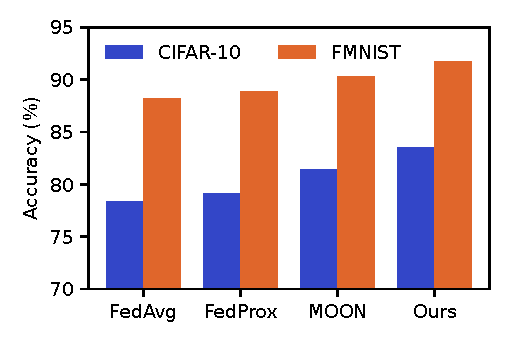
\includegraphics[width=\columnwidth]{figures/fig_accuracy.pdf}
\caption{Accuracy of all methods on CIFAR-10 and FMNIST.}
\label{fig:acc}
\end{figure}

As the number of clients grows, every method loses accuracy, but \ours{} degrades much more gracefully: with 100 clients it still reaches 80.2\%, while FedAvg drops to 75.1\% (Fig.~\ref{fig:clients}). We attribute this to the error feedback, which keeps the information that a single round's sketch cannot carry.

\begin{figure}[t]
\centering
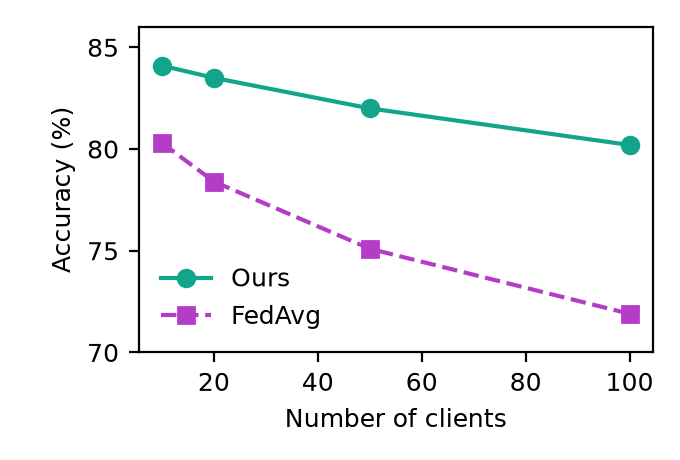
\includegraphics[width=\columnwidth]{figures/fig_clients.png}
\caption{Accuracy versus the number of clients}
\label{fig:clients}
\end{figure}

The sketch size matters less than expected. Fig.~\ref{fig:sketch} shows that accuracy saturates once each sketch has about 5000 columns, so the default of 8000 columns is a safe choice. We also observed that the RSE of the recovered update falls quickly with the sketch width, as shown in Fig.~\ref{fig:missing}.

\begin{figure}[t]
\centering
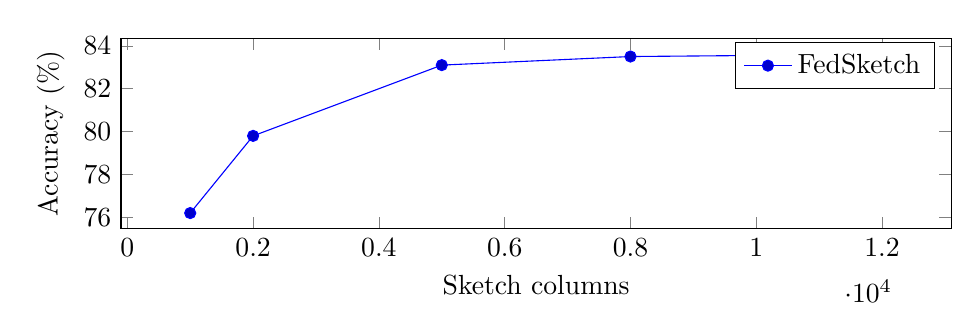
\begin{tikzpicture}
\begin{axis}[width=\columnwidth, height=4cm, xlabel={Sketch columns}, ylabel={Accuracy (\%)}]
\addplot coordinates {(1000,76.2) (2000,79.8) (5000,83.1) (8000,83.5) (12000,83.6)};
\legend{\ours}
\end{axis}
\end{tikzpicture}
\caption{Effect of the sketch width on CIFAR-10 accuracy.}
\label{fig:sketch}
\end{figure}

\section{Conclusion}
We presented \ours, a sketch-based compression scheme for federated learning that reaches 83.5\% accuracy on CIFAR-10 with 12 times less uplink traffic. Future work will study a adaptive sketch sizes during training and privacy guarantees with secure aggregation (SA).

\bibliographystyle{IEEEtran}
\bibliography{refs}
\end{document}
